% !TeX program = xelatex
\documentclass[aspectratio=169]{beamer}
\usepackage[english]{babel}
\usepackage{fontspec} % xelatex handles UTF-8 natively; inputenc is unneeded
\usepackage{csquotes}
\usepackage{amsmath,amssymb}
\usepackage{booktabs}
\usepackage{graphicx}
% \usepackage{expl3,biblatex}  % re-enable when you have a .bib
% \addbibresource{refs.bib}
\usetheme{metropolis}
\metroset{block=fill}

\title[Detach(): Stop-Gradient as Dynamics]{What Are We Optimizing When We Call \texttt{.detach()}?}
\subtitle[Stop-gradient and SSL]{Stop-gradient, self-supervised learning, and open research questions}
\author[Grunblat \& Arad]{Shoham Grunblat and Amit Arad}
\institute[Group Meeting]{Advisor: Assaf Shocher}
\date{\today}
\subject{Stop-gradient dynamics}
\keywords{stop-gradient, dynamics, Lyapunov, self-supervised learning}

\begin{document}

\begin{frame}[plain]
  \maketitle
\end{frame}

\begin{frame}{Outline}
  \tableofcontents
\end{frame}

% ============================================================
\section{The operator}
% ============================================================

\begin{frame}{One line of code, everywhere}
  \begin{columns}[T,onlytextwidth]
    \begin{column}{0.52\textwidth}
      \begin{block}{Forward --- transparent}
        \[ \mathrm{sg}(u) = u \]
      \end{block}
      \begin{block}{Backward --- opaque}
        \[ \nabla_u\,\mathrm{sg}(u) = 0 \]
      \end{block}
    \end{column}
    \begin{column}{0.44\textwidth}
      \texttt{.detach()} \quad \texttt{stop\_gradient}\\[0.6em]
      Self-distillation, TD learning, straight-through estimators, frozen
      teachers.\\[0.6em]
      Different learning tasks that share the use of \texttt{.detach()}.
    \end{column}
  \end{columns}

  \vspace{1em}
  \begin{center}
    \emph{What does it do to the optimization?}
  \end{center}
\end{frame}

% ============================================================
\section{What breaks}
% ============================================================

\begin{frame}{One dimension: the loss loses its authority}
  \[
    L(x) \;=\; \tfrac12 x^2 \;-\; \mathrm{sg}(x)\,x
  \]

  \begin{columns}[T,onlytextwidth]
    \begin{column}{0.46\textwidth}
      \begin{block}{The written loss}
        Forward, $\mathrm{sg}(x)=x$:
        \[ L(x) = -\tfrac12 x^2 \]
        Unbounded below.
      \end{block}
    \end{column}
    \begin{column}{0.46\textwidth}
      \begin{block}{The training field}
        Backward, the detached copy is frozen:
        \[ F(x) = x - x = 0 \]
        Training never moves.
      \end{block}
    \end{column}
  \end{columns}

  \vspace{0.8em}
  On an interval, every continuous 1-D field has a \alert{potential}.
  Here $F \equiv 0$, so its potential is constant.

  \vspace{0.3em}
  This potential differs from the forward loss.
\end{frame}

\begin{frame}{Two dimensions: the update has no potential}
  \[
    L(x,y) \;=\; x\,\mathrm{sg}(y) \;-\; y\,\mathrm{sg}(x)
    \qquad\Longrightarrow\qquad
    L \equiv 0 \ \ \text{identically}
  \]

  \vspace{0.4em}
  \begin{columns}[T,onlytextwidth]
    \begin{column}{0.52\textwidth}
      The field autodiff returns:
      \[ F = (y,\,-x), \qquad \dot\theta = -F \]
      Perfect circles. Forever.

      \vspace{0.8em}
      Clairaut's condition fails, so no function has $F$ as its gradient:
      \[ \partial_y F_x - \partial_x F_y = 1-(-1) = \alert{2} \neq 0 \]
    \end{column}
    \begin{column}{0.44\textwidth}
      \begin{center}
      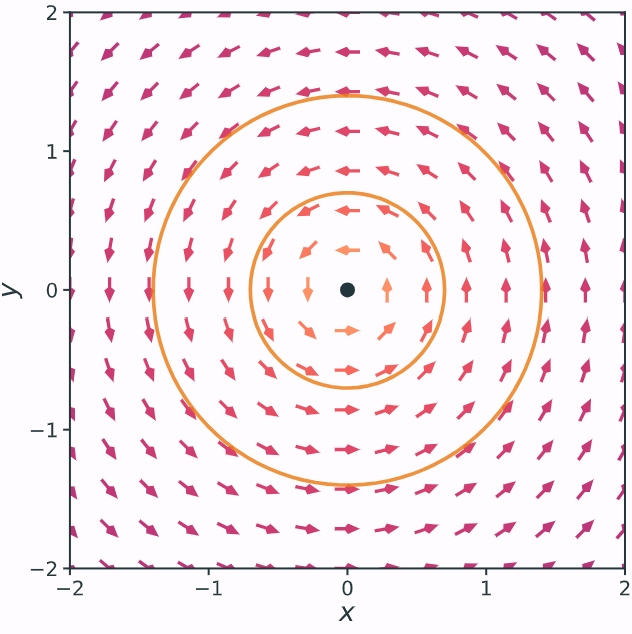
\includegraphics[width=\linewidth]{fig_circles.png}      \end{center}
    \end{column}
  \end{columns}

  \vspace{0.5em}
  A loss that is identically zero, and training that never stops moving.
\end{frame}

\begin{frame}{A game interpretation of this example}
  Back to $L = x\,\mathrm{sg}(y) - y\,\mathrm{sg}(x)$. Ask what each variable
  actually descends:

  \vspace{0.6em}
  \begin{columns}[T,onlytextwidth]
    \begin{column}{0.46\textwidth}
      \begin{block}{$x$ sees}
        \[ f_x(x) = x\,\bar y \qquad (\bar y \text{ frozen}) \]
        \[ \nabla_x f_x = \bar y \;=\; F_x \]
      \end{block}
    \end{column}
    \begin{column}{0.46\textwidth}
      \begin{block}{$y$ sees}
        \[ f_y(y) = -\,y\,\bar x \qquad (\bar x \text{ frozen}) \]
        \[ \nabla_y f_y = -\bar x \;=\; F_y \]
      \end{block}
    \end{column}
  \end{columns}

  \vspace{0.6em}
  \alert{Individual descent directions can produce joint cycles.}
\end{frame}

% ============================================================
% ============================================================
\begin{frame}{Stopping, improving, and staying nearby}
  Our circular game:
  \[
    \dot x=-y,\qquad \dot y=x,
    \qquad f_x=xy,\quad f_y=-xy.
  \]
  At the origin $(0,0)$:
  \begin{description}
    \item[Fixed point] $\dot x=\dot y=0$.
    \item[Nash equilibrium] $f_x(x,0)=f_y(0,y)=0$.\\
      Neither player can improve alone.
    \item[Stable, not attracting] Nearby trajectories stay on circles:
      \[
        x(t)^2+y(t)^2=r^2.
      \]
  \end{description}
  \begin{center}
    \alert{Staying nearby does not mean converging.}
  \end{center}
\end{frame}

\begin{frame}{Finding a Lyapunov function}
  Given the dynamics $\dot\theta=-F(\theta)$, seek a scalar $V$ with
  \[
    \dot V=-\nabla V^\top F\leq0.
  \]
  \begin{block}{Why look for one?}
    Strict decrease away from equilibria rules out cycles:
    returning to the same state would require the same $V$.
  \end{block}
\end{frame}
\section{Self-supervised learning}
% ============================================================

\begin{frame}{Learning without labels still needs a signal}
  Instead of human-provided labels, we construct a learning task
  from the data itself.

  \vspace{0.6em}
  One example: generate two augmented views of the same image,
  \[
    x_1 = t_1(x), \qquad x_2 = t_2(x),
  \]
  and encode them:
  \[
    z_1 = f_\theta(x_1), \qquad z_2 = f_\theta(x_2).
  \]

  \begin{block}{What we want}
    Representations that retain shared, useful information
    despite differences between the views.
  \end{block}

  But how do we turn this goal into a learning signal?
\end{frame}

\begin{frame}{Agreement alone admits a useless solution}
  A natural starting point is to bring the views together:
  \[
    L(\theta)
    = \mathbb{E}\big[
        \|f_\theta(x_1)-f_\theta(x_2)\|^2
      \big].
  \]

  \vspace{0.4em}
  But consider an encoder that returns the same vector
  for every input:
  \[
    f_\theta(x) \equiv c
    \qquad \Longrightarrow \qquad L(\theta)=0.
  \]

  \begin{alertblock}{Representation collapse}
    Perfect agreement, but no information that distinguishes inputs.
  \end{alertblock}

  \begin{center}
    How do we encourage agreement while avoiding collapse?
  \end{center}
\end{frame}
\section{The case that works: BYOL / SimSiam}
% ============================================================

\begin{frame}{Self-distillation: predict another view}
  Two augmented views of the same input: $x_1,x_2$.
  \[
    x_1\xrightarrow{\text{encoder }h_\theta}z_1
       \xrightarrow{\text{predictor }q_\phi}q_\phi(z_1)
  \]
  \[
    x_2\xrightarrow{\text{target encoder }h_{\bar\theta}}z_2
       \xrightarrow{\mathrm{sg}}\mathrm{sg}(z_2)
  \]
  \begin{block}{Learning signal}
    Make the online prediction match the stopped target.
  \end{block}
  \begin{center}
    \alert{How is the target encoder updated?}
  \end{center}
  {\small Here $h$ includes the encoder and projection head.}
\end{frame}

\begin{frame}{SimSiam and BYOL: where does the target come from?}
  \begin{block}{SimSiam: shared current weights}
    $\bar\theta=\theta$. Both views use the same encoder.\\
    The target output is detached for each directed loss.
  \end{block}
  \begin{block}{BYOL: a slowly moving target}
    A separate target encoder follows an exponential moving average:
    \[
      \bar\theta\leftarrow m\bar\theta+(1-m)\theta.
    \]
    Its weights are updated by averaging, not backpropagation.
  \end{block}
  Both use a predictor and swap the views to form a symmetric loss.
  \vfill
  {\scriptsize Grill et al., BYOL (2020); Chen and He, SimSiam (2021).}
\end{frame}

\begin{frame}{From a network to a scalar model}
  In a linear vector model:
  \[
    x_i\in\mathbb R^d,\quad W\in\mathbb R^{n\times d},
    \quad z_i=Wx_i\in\mathbb R^n,\quad P\in\mathbb R^{n\times n}.
  \]
  Here we choose $d=n=1$:
  \[
    x_1,x_2,w,p\in\mathbb R,\qquad
    z_i=wx_i,\quad pz_1=pwx_1.
  \]

\end{frame}

\begin{frame}{The scalar prediction task}
  \[
    \underbrace{pwx_1}_{\text{online prediction}}
    \quad\approx\quad
    \underbrace{\mathrm{sg}(wx_2)}_{\text{stopped target}}
  \]
  \[
    L_{\mathrm{code}}=\tfrac12\mathbb E
    \big[(pwx_1-\mathrm{sg}(wx_2))^2\big].
  \]
  Define
  \[
    k=\mathbb E[x_1^2]=\mathbb E[x_2^2]>0,
    \qquad s=\mathbb E[x_1x_2].
  \]
  \begin{center}
    $w,p$ are to be trained. \alert{$k,s$ are fixed data statistics.}
  \end{center}
\end{frame}

\begin{frame}{Deriving the predictor update}
  Write $e=pwx_1-wx_2$ for the numerical residual.
  The target does not depend on $p$, so
  \begin{align*}
    F_p&=\mathbb E[e\,wx_1]\\
       &=w^2\big(p\mathbb E[x_1^2]-\mathbb E[x_1x_2]\big)\\
       &=w^2(pk-s).
  \end{align*}
  Define $\beta=s-pk$. Gradient flow gives
  \[
    \boxed{\dot p=-F_p=w^2\beta.}
  \]
  \begin{center}
    For $w\ne0$, the predictor moves toward $p^\star=s/k$.
  \end{center}
\end{frame}

\begin{frame}{Deriving the encoder update: detach matters}
  During backpropagation, the target $wx_2$ is held fixed.
  Only the online prediction contributes:
  \begin{align*}
    F_w&=\mathbb E[e\,px_1]\\
       &=pw\big(p\mathbb E[x_1^2]-\mathbb E[x_1x_2]\big)\\
       &=pw(pk-s).
  \end{align*}
  Therefore
  \[
    \boxed{\dot w=-F_w=pw\beta.}
  \]
  \begin{center}
    Without detach, the residual derivative is $px_1-x_2$,
    rather than $px_1$.
  \end{center}
\end{frame}

\begin{frame}{Zero loss does not mean attraction}
  At collapse, $w=0$: prediction and target are both zero.
  \[
    L_{\mathrm{forward}}=0 \qquad \text{(a global minimum).}
  \]
  But a small encoder perturbation follows
  \[
    \dot w\approx aw,\qquad a=p_0(s-p_0k).
  \]
  If $s>0$ and $0<p_0<s/k$, then $a>0$:
  \[
    w(t)\approx w(0)e^{at}.
  \]
  \begin{center}
    \alert{The detached update can push away from a loss minimum.}
  \end{center}
\end{frame}

\begin{frame}{Finding a decreasing quantity}
  The predictor mismatch is $\beta=s-pk$.
  With fixed $s,k$,
  \[
    \dot\beta=-k\dot p=-kw^2\beta.
  \]
  Choose $V(p,w)=\beta^2$. Then
  \[
    \boxed{\dot V=2\beta\dot\beta=-2kw^2\beta^2\leq0.}
  \]
  \begin{center}
    \alert{A decreasing residual, despite a generally non-gradient field.}
  \end{center}
  {\small Indeed $\partial_w\dot p-\partial_p\dot w=ws$,
  which is nonzero when $ws\ne0$.}
\end{frame}

\begin{frame}{Training can stop for two different reasons}
  \[
    \dot V=-2kw^2\beta^2=0
    \quad\Longleftrightarrow\quad
    \beta=0\ \text{or}\ w=0.
  \]
  \begin{block}{The predictor reaches its preferred scale}
    $\beta=0$: $p=s/k$.
  \end{block}
  \begin{block}{The encoder outputs nothing}
    $w=0$: prediction and target vanish; all updates stop.
  \end{block}
  \begin{center}
    \alert{A decreasing mismatch does not distinguish learning from collapse.}
  \end{center}
\end{frame}

\begin{frame}{An invariant can rule out collapse in the toy model}
  The scalar equations conserve
  \[
    p(t)^2-w(t)^2=p(0)^2-w(0)^2.
  \]
  For example, choose $p(0)=0$ and $w(0)=1$. Then
  \[
    p(t)^2-w(t)^2=-1
    \quad\Longrightarrow\quad w(t)^2=p(t)^2+1\geq1.
  \]
  \begin{center}
    \alert{This initialization cannot reach a collapsed encoder.}
  \end{center}
  \vspace{0.5em}
  {\small This is a scalar-model conclusion. In higher dimensions,
  feature directions can interact and some may collapse.}
  \begin{center}
    What comparable guarantees survive in richer models?
  \end{center}
\end{frame}

% ============================================================
\section{PEIRA}

\begin{frame}{From the toy example to PEIRA}
  Our introduction raised three questions:
  \begin{enumerate}
    \item Do the stop-gradient training dynamics converge?
    \item Which representations do they reach?
    \item Can collapse be stable?
  \end{enumerate}
  \begin{center}
    \alert{Beyond the scalar example: what can we prove about self-distillation?}
  \end{center}
  {\small Arbel, Terver and Ponce (2026),
  \emph{Learning Predictive Encoders through Inter-View Regressor Alignment}.}
\end{frame}

\begin{frame}{The baseline: two encoders and a predictor}
  Paired inputs: $x\in\mathbb R^{d_1}$, $y\in\mathbb R^{d_2}$.
  \[
    \underbrace{U(x),\ V(y)\in\mathbb R^k}_{\text{nonlinear encoders' representations}},
    \qquad
    \underbrace{P\in\mathbb R^{k\times k}}_{\text{linear predictor}}.
  \]
  Each encoder predicts the other view:
  \[
    P\,U(x)\approx\mathrm{sg}(V(y)),\qquad
    P\,V(y)\approx\mathrm{sg}(U(x)).
  \]
  Gradients pass through each prediction branch, not its target.
  \vspace{0.6em}
  \begin{center}
    \alert{Whenever the encoders change, the predictor is solved exactly.}
  \end{center}
\end{frame}

\begin{frame}{CCA: finding what two views share}
  Across many paired views, look for two features:
  \[
    a=\psi(x),\qquad b=\xi(y).
  \]
  \begin{itemize}
    \item Choose features whose outputs vary together most strongly.
    \item Normalize their scale for a fair comparison.
    \item Find another pair that does not repeat earlier features.
  \end{itemize}
  \begin{center}
    \alert{Nonlinear CCA gives ordered pairs of shared features.}
  \end{center}
  {\small CCA = canonical correlation analysis. Each feature sees only its own view.}
\end{frame}

\begin{frame}{How does PEIRA use CCA?}
  Each canonical pair has a shared-signal strength $c_i$:
  \[
    \mathbb E[\psi_i(x)\xi_j(y)]
      =\begin{cases}c_i,&i=j,\\0,&i\ne j.\end{cases}
  \]
  Different pairs have no cross-correlation.
  \begin{itemize}
    \item Express the encoders using these shared directions.
    \item Identify which directions occur at equilibria.
    \item Test whether missing directions grow under perturbations.
  \end{itemize}
  \begin{center}
    \alert{CCA describes the learned representation; it is not a preprocessing step.}
  \end{center}
\end{frame}

\begin{frame}{From analyzing self-distillation to changing the objective}
  \begin{enumerate}
    \item \textbf{CCA:} identify shared feature directions;
          describe equilibria and analyze their stability.
    \item \textbf{Lyapunov certificate:} construct a decreasing quantity
          from representation statistics to help prove convergence.
    \item \textbf{The problem:} convergence can still end in zero
          or partial collapse.
    \item \textbf{The response:} design PEIRA's objective so stable equilibria
          retain the leading eligible directions.
  \end{enumerate}
  \vspace{0.5em}
  \begin{center}
    \alert{Analyze what training reaches, then change what it rewards.}
  \end{center}
\end{frame}

\begin{frame}{PEIRA: a new objective with better stable outcomes}
  Let $P^\star$ be the best regularized cross-view predictor.
  \[
    \mathcal E_{\mathrm{PEIRA}}
    =\underbrace{-\tfrac12\operatorname{Tr}(P^\star)}_{\text{reward shared predictive structure}}
     +\underbrace{\tfrac\lambda2
       \mathbb E[\|U(x)\|^2+\|V(y)\|^2]}_{\text{control representation scale}}.
  \]
  $\operatorname{Tr}$ denotes the matrix trace.
  \begin{itemize}
    \item Stable equilibria are global minimizers.
    \item They retain the strongest eligible CCA directions,
          up to the representation's capacity.
  \end{itemize}
  \begin{center}
    \alert{Stable solutions retain the strongest shared features allowed by regularization and representation size.}
  \end{center}
\end{frame}
\section{Possible research directions}

\begin{frame}{Research questions: from one model to a general method}
  \begin{enumerate}
    \item \textbf{Starting point: finite-speed predictor.}\\
      Can we extend PEIRA's self-distillation certificate when the
      predictor learns alongside the encoders?
    \item \textbf{Constructive certificates.}\\
      Can residuals and tracking errors guide the construction
      of a Lyapunov function?
    \item \textbf{Generalization.}\\
      Which structural conditions let the same construction
      work across different stop-gradient models?
    \item \textbf{Beyond convergence.}\\
      Can we also determine when collapse attracts or repels,
      and which features survive?
  \end{enumerate}
\end{frame}
% \section{\bibname}
% \begin{frame}[t, allowframebreaks]{\bibname}
%   \printbibliography[heading=none]
% \end{frame}

\begin{frame}[plain]
  \vfill
  \centerline{\Large Thank you --- questions?}
  \vfill\vfill
\end{frame}

% ============================================================
\appendix
% ============================================================


\end{document}




































